
% *** Authors should verify (and, if needed, correct) their LaTeX system  ***
% *** with the testflow diagnostic prior to trusting their LaTeX platform ***
% *** with production work. The IEEE's font choices and paper sizes can   ***
% *** trigger bugs that do not appear when using other class files.       ***                          ***
% The testflow support page is at:
% http://www.michaelshell.org/tex/testflow/



\documentclass[conference]{IEEEtran}
% Some Computer Society conferences also require the compsoc mode option,
% but others use the standard conference format.
%
% If IEEEtran.cls has not been installed into the LaTeX system files,
% manually specify the path to it like:
% \documentclass[conference]{../sty/IEEEtran}





% Some very useful LaTeX packages include:
% (uncomment the ones you want to load)


% *** MISC UTILITY PACKAGES ***
%
%\usepackage{ifpdf}
% Heiko Oberdiek's ifpdf.sty is very useful if you need conditional
% compilation based on whether the output is pdf or dvi.
% usage:
% \ifpdf
%   % pdf code
% \else
%   % dvi code
% \fi
% The latest version of ifpdf.sty can be obtained from:
% http://www.ctan.org/pkg/ifpdf
% Also, note that IEEEtran.cls V1.7 and later provides a builtin
% \ifCLASSINFOpdf conditional that works the same way.
% When switching from latex to pdflatex and vice-versa, the compiler may
% have to be run twice to clear warning/error messages.






% *** CITATION PACKAGES ***
%
%\usepackage{cite}
% cite.sty was written by Donald Arseneau
% V1.6 and later of IEEEtran pre-defines the format of the cite.sty package
% \cite{} output to follow that of the IEEE. Loading the cite package will
% result in citation numbers being automatically sorted and properly
% "compressed/ranged". e.g., [1], [9], [2], [7], [5], [6] without using
% cite.sty will become [1], [2], [5]--[7], [9] using cite.sty. cite.sty's
% \cite will automatically add leading space, if needed. Use cite.sty's
% noadjust option (cite.sty V3.8 and later) if you want to turn this off
% such as if a citation ever needs to be enclosed in parenthesis.
% cite.sty is already installed on most LaTeX systems. Be sure and use
% version 5.0 (2009-03-20) and later if using hyperref.sty.
% The latest version can be obtained at:
% http://www.ctan.org/pkg/cite
% The documentation is contained in the cite.sty file itself.






% *** GRAPHICS RELATED PACKAGES ***
%
\ifCLASSINFOpdf
  \usepackage[pdftex]{graphicx}
  % declare the path(s) where your graphic files are
  \graphicspath{{../pdf/}{../jpeg/}}
  % and their extensions so you won't have to specify these with
  % every instance of \includegraphics
  \DeclareGraphicsExtensions{.pdf,.jpeg,.png}
\else
  % or other class option (dvipsone, dvipdf, if not using dvips). graphicx
  % will default to the driver specified in the system graphics.cfg if no
  % driver is specified.
  \usepackage[dvips]{graphicx}
  % declare the path(s) where your graphic files are
  \graphicspath{{../eps/}}
  % and their extensions so you won't have to specify these with
  % every instance of \includegraphics
  \DeclareGraphicsExtensions{.eps}
\fi
% graphicx was written by David Carlisle and Sebastian Rahtz. It is
% required if you want graphics, photos, etc. graphicx.sty is already
% installed on most LaTeX systems. The latest version and documentation
% can be obtained at: 
% http://www.ctan.org/pkg/graphicx
% Another good source of documentation is "Using Imported Graphics in
% LaTeX2e" by Keith Reckdahl which can be found at:
% http://www.ctan.org/pkg/epslatex
%
% latex, and pdflatex in dvi mode, support graphics in encapsulated
% postscript (.eps) format. pdflatex in pdf mode supports graphics
% in .pdf, .jpeg, .png and .mps (metapost) formats. Users should ensure
% that all non-photo figures use a vector format (.eps, .pdf, .mps) and
% not a bitmapped formats (.jpeg, .png). The IEEE frowns on bitmapped formats
% which can result in "jaggedy"/blurry rendering of lines and letters as
% well as large increases in file sizes.
%
% You can find documentation about the pdfTeX application at:
% http://www.tug.org/applications/pdftex





% *** MATH PACKAGES ***
%
\usepackage{amsmath}
% A popular package from the American Mathematical Society that provides
% many useful and powerful commands for dealing with mathematics.
%
% Note that the amsmath package sets \interdisplaylinepenalty to 10000
% thus preventing page breaks from occurring within multiline equations. Use:
%\interdisplaylinepenalty=2500
% after loading amsmath to restore such page breaks as IEEEtran.cls normally
% does. amsmath.sty is already installed on most LaTeX systems. The latest
% version and documentation can be obtained at:
% http://www.ctan.org/pkg/amsmath





% *** SPECIALIZED LIST PACKAGES ***
%
%\usepackage{algorithmic}
% algorithmic.sty was written by Peter Williams and Rogerio Brito.
% This package provides an algorithmic environment fo describing algorithms.
% You can use the algorithmic environment in-text or within a figure
% environment to provide for a floating algorithm. Do NOT use the algorithm
% floating environment provided by algorithm.sty (by the same authors) or
% algorithm2e.sty (by Christophe Fiorio) as the IEEE does not use dedicated
% algorithm float types and packages that provide these will not provide
% correct IEEE style captions. The latest version and documentation of
% algorithmic.sty can be obtained at:
% http://www.ctan.org/pkg/algorithms
% Also of interest may be the (relatively newer and more customizable)
% algorithmicx.sty package by Szasz Janos:
% http://www.ctan.org/pkg/algorithmicx




% *** ALIGNMENT PACKAGES ***
%
%\usepackage{array}
% Frank Mittelbach's and David Carlisle's array.sty patches and improves
% the standard LaTeX2e array and tabular environments to provide better
% appearance and additional user controls. As the default LaTeX2e table
% generation code is lacking to the point of almost being broken with
% respect to the quality of the end results, all users are strongly
% advised to use an enhanced (at the very least that provided by array.sty)
% set of table tools. array.sty is already installed on most systems. The
% latest version and documentation can be obtained at:
% http://www.ctan.org/pkg/array


% IEEEtran contains the IEEEeqnarray family of commands that can be used to
% generate multiline equations as well as matrices, tables, etc., of high
% quality.




% *** SUBFIGURE PACKAGES ***
\ifCLASSOPTIONcompsoc
  \usepackage[caption=false,font=normalsize,labelfont=sf,textfont=sf]{subfig}
\else
  \usepackage[caption=false,font=footnotesize]{subfig}
\fi
% subfig.sty, written by Steven Douglas Cochran, is the modern replacement
% for subfigure.sty, the latter of which is no longer maintained and is
% incompatible with some LaTeX packages including fixltx2e. However,
% subfig.sty requires and automatically loads Axel Sommerfeldt's caption.sty
% which will override IEEEtran.cls' handling of captions and this will result
% in non-IEEE style figure/table captions. To prevent this problem, be sure
% and invoke subfig.sty's "caption=false" package option (available since
% subfig.sty version 1.3, 2005/06/28) as this is will preserve IEEEtran.cls
% handling of captions.
% Note that the Computer Society format requires a larger sans serif font
% than the serif footnote size font used in traditional IEEE formatting
% and thus the need to invoke different subfig.sty package options depending
% on whether compsoc mode has been enabled.
%
% The latest version and documentation of subfig.sty can be obtained at:
% http://www.ctan.org/pkg/subfig




% *** FLOAT PACKAGES ***
%
%\usepackage{fixltx2e}
% fixltx2e, the successor to the earlier fix2col.sty, was written by
% Frank Mittelbach and David Carlisle. This package corrects a few problems
% in the LaTeX2e kernel, the most notable of which is that in current
% LaTeX2e releases, the ordering of single and double column floats is not
% guaranteed to be preserved. Thus, an unpatched LaTeX2e can allow a
% single column figure to be placed prior to an earlier double column
% figure.
% Be aware that LaTeX2e kernels dated 2015 and later have fixltx2e.sty's
% corrections already built into the system in which case a warning will
% be issued if an attempt is made to load fixltx2e.sty as it is no longer
% needed.
% The latest version and documentation can be found at:
% http://www.ctan.org/pkg/fixltx2e


%\usepackage{stfloats}
% stfloats.sty was written by Sigitas Tolusis. This package gives LaTeX2e
% the ability to do double column floats at the bottom of the page as well
% as the top. (e.g., "\begin{figure*}[!b]" is not normally possible in
% LaTeX2e). It also provides a command:
%\fnbelowfloat
% to enable the placement of footnotes below bottom floats (the standard
% LaTeX2e kernel puts them above bottom floats). This is an invasive package
% which rewrites many portions of the LaTeX2e float routines. It may not work
% with other packages that modify the LaTeX2e float routines. The latest
% version and documentation can be obtained at:
% http://www.ctan.org/pkg/stfloats
% Do not use the stfloats baselinefloat ability as the IEEE does not allow
% \baselineskip to stretch. Authors submitting work to the IEEE should note
% that the IEEE rarely uses double column equations and that authors should try
% to avoid such use. Do not be tempted to use the cuted.sty or midfloat.sty
% packages (also by Sigitas Tolusis) as the IEEE does not format its papers in
% such ways.
% Do not attempt to use stfloats with fixltx2e as they are incompatible.
% Instead, use Morten Hogholm'a dblfloatfix which combines the features
% of both fixltx2e and stfloats:
%
% \usepackage{dblfloatfix}
% The latest version can be found at:
% http://www.ctan.org/pkg/dblfloatfix




% *** PDF, URL AND HYPERLINK PACKAGES ***
%
%\usepackage{url}
% url.sty was written by Donald Arseneau. It provides better support for
% handling and breaking URLs. url.sty is already installed on most LaTeX
% systems. The latest version and documentation can be obtained at:
% http://www.ctan.org/pkg/url
% Basically, \url{my_url_here}.




% *** Do not adjust lengths that control margins, column widths, etc. ***
% *** Do not use packages that alter fonts (such as pslatex).         ***
% There should be no need to do such things with IEEEtran.cls V1.6 and later.
% (Unless specifically asked to do so by the journal or conference you plan
% to submit to, of course. )


% correct bad hyphenation here
\hyphenation{}


\begin{document}
% Title ideas here:

\title{Exploiting the Graph: Increasing Engagement in Collaborative Interactive Evolution}



\author{\IEEEauthorblockN{Michael Shell}
\IEEEauthorblockA{School of Electrical and\\Computer Engineering\\
Georgia Institute of Technology\\
Atlanta, Georgia 30332--0250\\
Email: http://www.michaelshell.org/contact.html}
\and
\IEEEauthorblockN{Homer Simpson}
\IEEEauthorblockA{Twentieth Century Fox\\
Springfield, USA\\
Email: homer@thesimpsons.com}
\and
\IEEEauthorblockN{James Kirk\\ and Montgomery Scott}
\IEEEauthorblockA{Starfleet Academy\\
San Francisco, California 96678--2391\\
Telephone: (800) 555--1212\\
Fax: (888) 555--1212}}

\maketitle

% As a general rule, do not put math, special symbols or citations
% in the abstract
\begin{abstract}
Interactive evolution is the leading technique employed by 
Evolutionary Art researchers, where users' preferences guide the search. A common
practice is to develop Interactive Evolutionary Computation (IEC) algorithms
as web applications in order to give users easy access the application as they
often depend on volunteers who visit the system to interactively help with the search. 
There are several drawbacks that limit user participation 
such as human fatigue and boredom resulting from evaluating 
a large number of individuals. 
To tackle this issues, we propose the design of IEC systems using a human-centered 
approach, with a framework consisting of a social network of 
volunteers, interacting with a population consisting also of a network 
of individuals. In this work we propose a graph model as a practical 
and efficient tool for mapping in a natural way the relationships 
found in the system. A case study is presented as a proof of concept, 
providing both conceptual and implementation details of a graph based model 
as it is  applied in the implementation of an IEA using the EvoSpace-Interactive platform. 
As a result, the graph model was successfully applied in a gamification technique 
developed to increase user engagement. 



%and novelty. % These two last issues are not too clear, maybe they
             % could be explained in that motivation. 

\end{abstract}

% no keywords
\IEEEpeerreviewmaketitle



\section{Introduction}
Interactive Evolutionary Algorithms (IEAs) are standard EAs whose
fitness evaluations are performed by persons within an interactive 
system.  Thus, the main loop of the EA needs the intervention of a
human to perform the quality assessment of each proposed solution.
IEAs have demonstrated their ability for effectively
producing art and design \cite{Bentley:1999:intro,Sims:1991,todd:1992},
as well as other products in many other domains \cite{ie1}. 
Several IECs have been developed as web based systems \cite{picbreeder},
who depend on volunteers who visit the system to interactively help
with the search, using both anonymous and registered users.
These systems have several inherent drawbacks arising from the very nature of 
the algorithms, namely, the human fatigue caused by the interaction, and
the boredom arising when users evaluate a large number of individuals 
many of which are not interesting or are very similar to each other.
IEAs also share some of the issues commonly found in volunteer based systems
\cite{sarmenta2001volunteer,web:BOINC} such as the volunteer\'s lack of accountability,
and the need to build trust between participants and application providers. 
For the provider there is also the difficulty of establishing 
the amount of time and resources
a volunteer is willing to spend on the system, and how they decide if they
participate or not \cite{JJ:2016}. In order to increase participation and 
engagement, and to tackle the issues mentioned above,  
IEAs must follow a human centered design, giving extensive attention 
to volunteer users, not only because their
explicit evaluation is essential, but also because the context of the 
interaction affects the system as a whole. Users interact not only with the graphical
interface, and each individual\'s phenotype, there is also the interaction
with other users, their previous evaluations and their own stream of activities
and past experiences. Thus users in this proposal are defined as dynamic entities 
interacting with an evolutionary computation having the fundamental purpose 
of evaluating individuals according to their preferences,
both explicitly or implicitly. In this work we propose giving the same
importance to users and their interactions as the population of 
individuals have in a traditional EA, even to the extend as using this
knowledge as an integral part of the evolutionary algorithm. We argue also
that a graph model is a viable representation for this purpose,  
presenting a natural way of mapping the relationships found in the system. 
Most IEAs have the following many-to-many relations:

\begin{itemize}

  \item {\bf Individual-Individual} The relationships between individuals in the
  population are naturally expressed as a tree, or a graph when both ancestors 
  and descendants are considered. Other semantic relations can also be of interest
  for instance similarity or composition.


  \item {\bf User-Individual}
  Many kind of relationships between users and individuals,
  can be expressed using common actions found in social networks;
  for instance: share, like, rate or add to collection \cite{Prodromou:16:AS}. In IEAs these
  relationships are used to assign a single or a collection of
  fitness values to individuals \cite{garcia2013evospace}.   

  \item {\bf User-User}
  Relationship between users can also be modeled 
  as a social network, with well established semantics, algorithms and metrics \cite{ahuja1993network}.
  A graph model could enable researchers to find other ways of identifying leaders of 
  opinion or measuring the similarity between user's preferences. 
  These measures can then be used by recommender algorithms selecting 
  individuals according users' preferences. 

\end{itemize}

These relations are naturally mapped to graphs, while other actions and 
properties can also be modeled as a semantic network using
basic subject–-predicate-–object expressions \cite{Prud'hommeaux:14:RT}.
Another reason for using a graph model is the tools available for
implementing and query the model, and the increased performance of
native graph database systems \cite{holzschuher2013performance,holzschuher2016querying}.


% Moving to related work - Mario
%\cite{Performance for the masses and Christian's previous work}, 



 % Can it be quantified? Maybe a reference to NodIO? - JJ
%Some authors have already tried to address this basic problem
%\cite{Frade:2010:EvoGAMES}. %Non sequitur. Is it something we are
                            %going to do here? - jj
%% Moving this to Related Work Section -Mario
% That section is not there yet. Forgot to paste? - JJ

 
A case study is presented as a proof of concept, providing both
conceptual and implementation details of a graph data model applied in the 
implementation of an IEA. The experiment was implemented using
the EvoSpace-Interactive framework, and consisted of a web application
for evolving artistic drawings. The graph database is then used to
measure the degree of relationship between users and their participation.  

The remainder of this paper is organized as follows.
Section \ref{sec:interactive} presents related work on the topic 
of Interactive Evolution with emphasis in data models.
Then, Section \ref{sec:evospace-i} presents the computational platform on which 
the main proposal of this work is developed. The proposed graph model is 
presented in Section \ref{sec:graph}.
The experimental work and results are presented in Section \ref{sec:experiments}.
Finally, a concluding remarks are provided in Section \ref{sec:conclusions}.


\section{Related Work}
\label{sec:interactive}
% IEC 
% Collaborative
% Users - Volunteers - Engagement
% Too much data
% Relational MySQL, Key-Value, Mongo, Redis, Memcached
% Not well suited for certain relations.
% Graph DBs, Performance, Query Langs 
% Are they any good? 
% Titan, Neo4J

The IEC the approach has been used in a wide variety of applications and problem domains
and remains an active area of research. However, in this work, emphasis is given to IEAs 
implemented as volunteer based collaborative systems; where volunteers interact and evaluate 
an evolving population, thus guiding the search based on an aggregate their subjective 
preferences. What follows is not intended as a comprehensive survey, only a review of 
the most relevant contributions to the present work, with special attention put in
data structures and data management requirements.

From the earlier works in the IEC field the notion of user collaboration in a natural way
has been proposed. A notable application was the Galapagos Project \cite{sims1997interactivity},
an exhibit in the Tokyo Multimedia Museum (1997--2000) were visitors interacted with images presented in 
twelve displays by selecting those they find most aesthetically interesting by standing on
step sensors in front of each. An early example of web based collaboration is the work by 
Langdon \cite{langdon:2004}, evolving fractal representations of virtual creatures. It proposed a distributed 
EA using a global population stored on a central web server sending 
portions of the population to remote clients using JavaScript. Users evaluated individuals locally 
and returned to the server those they liked more, to be distributed over the web.
Similarly, Secretan et al. \cite{picbreeder} and Clune and Lipson \cite{forms} use web-based IEAs 
to evolve artistic artifacts using a generative encoding, compositional pattern producing networks.

In all these systems, the evolutionary interactive process is captured by the system. The genetic lineage of each
individual is presented where users can visualize the relationships between them and evolutionary operators used in
their creation. Also there is information regarding users and their collaborations.  Common offerings show 
interesting individuals order by categories, number of votes, best of the week among others.
These features have the goal of encouraging participation but require the use of a database system 
for their implementation. Picbreeder \cite{picbreeder} is implemented with a service oriented
architecture using a relational database and the file system for genotypes and images. 

Collaborative IEC systems need to store highly connected data, as it is common in current applications
like social networks, and the world wide web. In order to deal with large datasets of connected data,
graph databases \cite{angles2012comparison} have been proposed as an alternative to relational databases 
which have performance limitations when dealing with highly connected data \cite{holzschuher2013performance}.

The present work builds on a previous proposals and extends the C-IEA approach.
First, it proposes a graph data model for representing the interactive process of C-IEC systems.
Second, it incorporates the graph model to the evolutionary algorithm.
Finally, uses the same model to increase the collaboration of volunteers.


\section{EvoSpace-Interactive}
\label{sec:evospace-i}
\begin{figure}[!t]
    \centering
        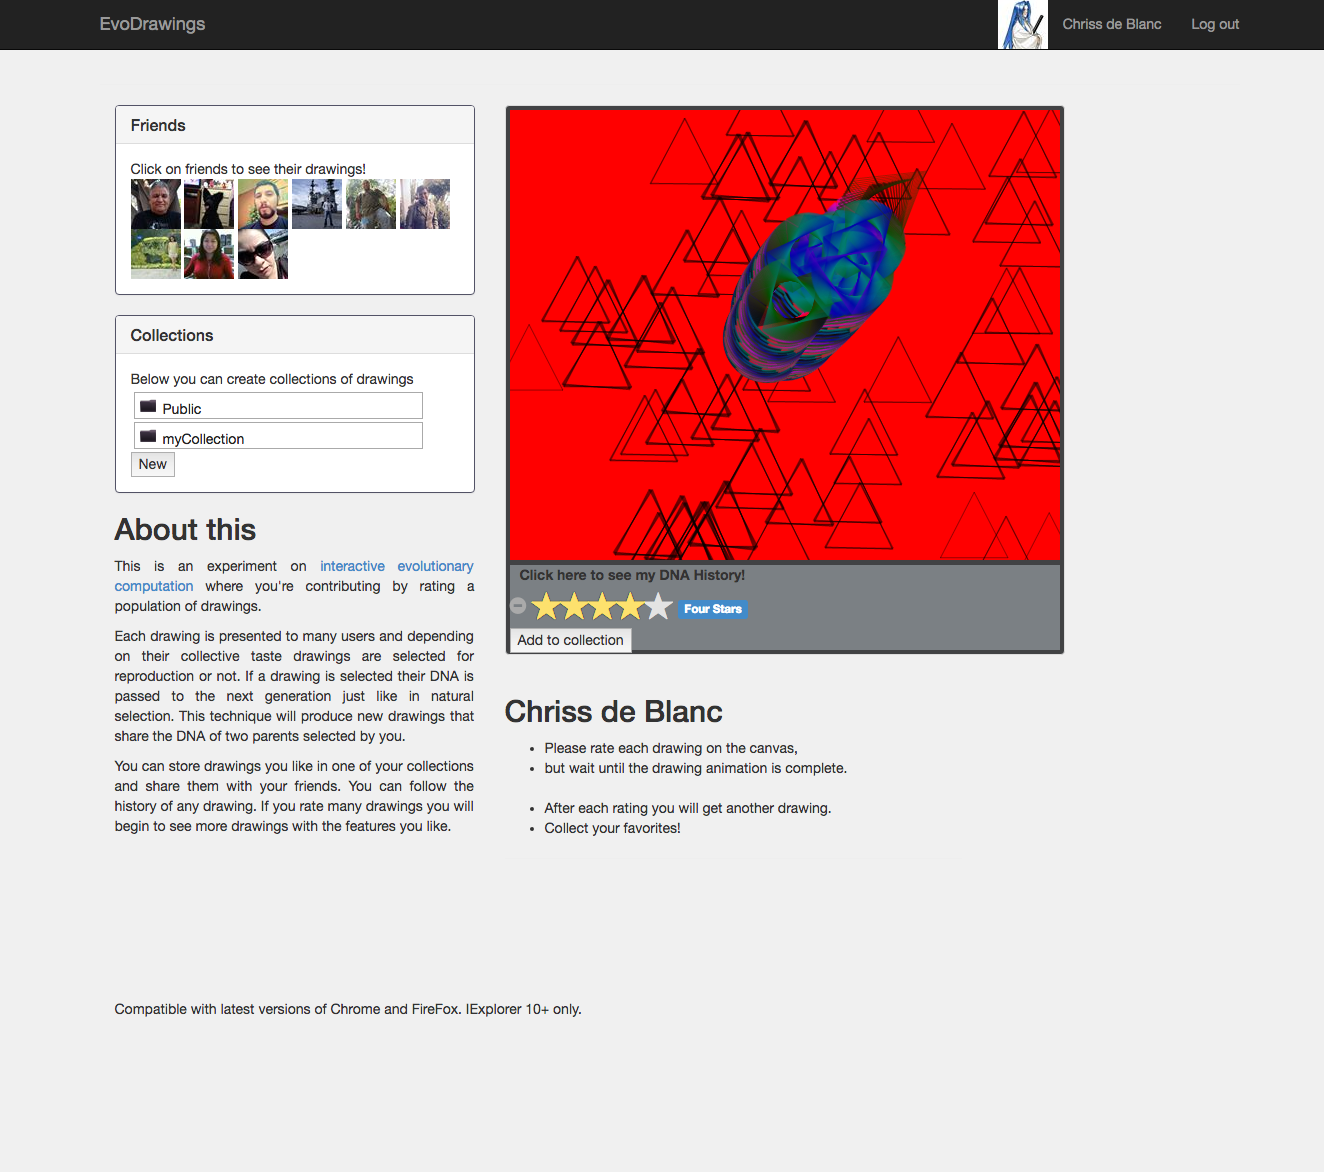
\includegraphics[width=3.5in]{img/UI_ed01.png}
    \caption{User interface of an EvoSpace-Interactive application.}
    \label{fig:web}
\end{figure}

As a case study, a IEA was developed using the 
EvoSpace-Interactive (ES-I) platform \cite{garcia2013evospace}. %citation
A brief description of the application is presented next, focusing
on the data elements that where ported to the graph model.

\subsection{Fitness Assignment}
\label{sec:assignment}
The ES-I platform employs a collaborative technique,
where several registered users assign a quality assessment to a single
individual and then an aggregated fitness value is calculated. The fitness
assigned to each individual depends on the taste of each particular user, 
resulting in a many-to-many relationship between users and individuals. 
Many systems query this user-individual relation to extract relevant
knowledge about the process and the population, for instance showing the
most popular individual, or the the user with more participation 
\cite{picbreeder}.
In order to do this, data about individuals 
must be permanently stored, even
if they are no longer in the active population. 

\subsection{Collaboration}
\label{sec:col}
After entering the web application by using their Facebook account,
users can collaborate with their Facebook friends, 
sharing those individuals they like, or by taking individuals
from their friend\'s collections by using the web interface depicted 
in Figure \ref{fig:web}.
At the top left corner a list of Facebook friends is presented
to encourage users to interact with the system. In the central 
\emph{ Wall } area, an individual sampled from the population that is
being evolved via the evolutionary algorithm 
is shown to the user.
Here, the user can interact with the system in two ways.
He can assign a quality assessment to the individual using
a five star rating measure.
Additionally, a user can choose to add an image to one of their \emph{Collections}.
A collection is a special directory to store individuals a user prefers and wishes
to save. After the user finishes interacting the individual
on the Wall, he can choose to retrieve a new one from population.
At the left side, is the \emph{Collections} section.
The user can create several collections, to group and organize his favorite 
artifacts. Moreover, a user can browse the content of each collection and from
there share images through the social network.
When a user browses over an individual a detail pane shows how many users have
liked the individual. The pane also includes a link to the individual's 
details, the parents, genetic operators that created it, and genealogy information.

\begin{figure*}[!t]
    \centering
        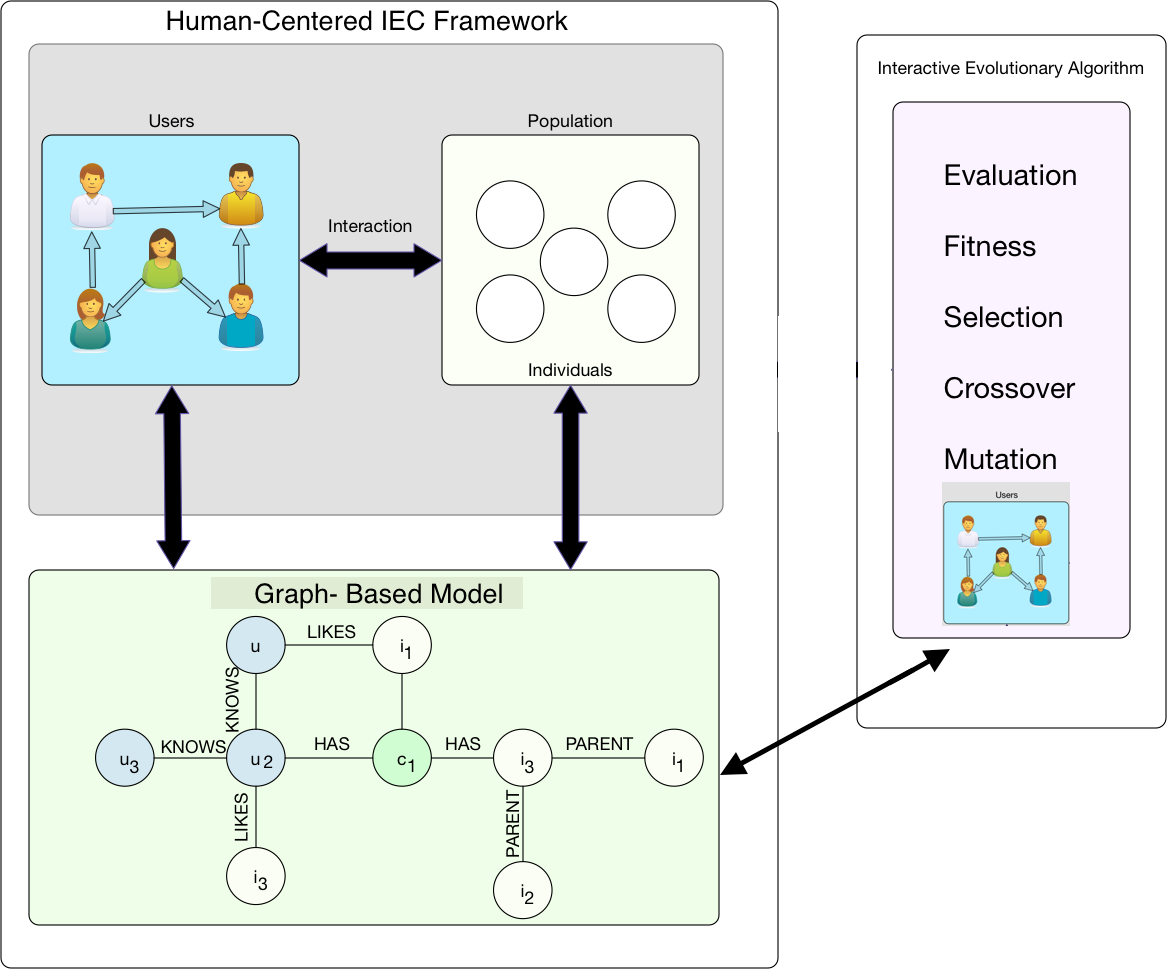
\includegraphics[width=3.5in]{img/framework.png}
    \caption{IEC Human-centered framework.}
    \label{fig:uc_framework}
\end{figure*}


 \section{IEC Human-centered framework}
\label{sec:graph}
The general goal of this research is to develop a human-centered \cite{gasson2003human} framework
for interactive evolutionary computation (IEC) in order to increase
participation and also to minimize the amount of evaluations needed for the
evolutionary process in given IEC application. We deliberately use the 
more general
term Human instead of User, because humans are not always playing the role of
users in software engineering sense, they could just be interacting 
naturally with their environment and with out knowing they are implicitly
evaluating a possible solution. In other cases the evaluation could be done
by the natural interactions of a group of humans in a collaborative fashion
or not. For instance the IEC algorithm could by trying to optimize 
the design of an exit sign in an airport, then the quality of this sign could be
determined by the average the time it takes a sample of people to 
find the exit. In this example there could be certain collaboration
between users if they are not traveling alone, of course this is only one of
the considerations designers could make. 


The human centered framework consists of three high level components depicted
in figure \ref{fig:uc_framework}:

\begin{itemize}
  \item {\bf Interactive Evolutionary Computational system} 
  This is the real world system that we are going to represent in the model, 
  it consist of human users and their interactions with one or more individuals
  from
  the population. There are many ways in which humans could interact 
  with individuals, this could be through a mobile device, a user interface 
  or by interacting with real world objects generated as part of the algorithm 
  \cite{de2014artists,de2013unplugging}. 
  There is also the possibility that fitness or even part of the search 
  to be done by devices lent by the human \cite{merelo2016performance}.
  The information gathered through the interaction is the primary concern
  as it will guide the search. 

  \item {\bf IEC Data Model}
  A data model is used to describe the IEC system prior to a physical 
  implementation. 
  %% This block is maybe not needed but in our ES-I implementation
  %% we use Relational (PosgreSQL), Objects (JSON-Redis) and Graphs (Neo4J)
  Depending on the domain several techniques can be used.
  Parts of the system could be better described by an Entity relationship 
  modeling to be used in a relational database or a Class Digram for a 
  key-value store. 
  %%
  %%
  A graph is proposed for modeling the social network
  of users and their interaction with the population. This database 
  is the back-end of the system, is used by the EA and the user interface. 

  \item {\bf Evolutionary Algorithm} 
  The EA algorithm queries the graph model, and then updates those nodes that 
  are part of the population. The EA could also be done with the help of
  humans, for instance in the XY project \cite{de2013unplugging} artists physically created
  the new population.  
\end{itemize}

\section{IEC Graph Data Model} 

A graph is composed of two fundamental entities: nodes and relationships,
both having attributes. Nodes are abstractions of the objects in the real 
world system, and relationships describe their interactions. Types describe
the attributes describing an entity, First we describe the types of nodes and
relationships in the system. 

\subsection{Node Types}
\begin{itemize}

\item {\bf Users} This nodes represent the human users of the system and have 
the attributes: {\tt id} a unique identifier, {\tt name}  and {\tt created}
specifying the  creation date (time stamp) of the node. 

\item {\bf Individual} This type of node has the following attributes: 
{\tt id}, {\tt chromosome}  and {\tt views} this is 
the amount that users have seen or interacted with this individual and
 {\tt created}.

\item {\bf Collection} This type of nodes represent the collections belonging
to users, their attributes are {\tt id}, 
{\tt name}, {\tt created} and {\tt is\_private} indicating if this collection
contents can be are shared with others. 
\end{itemize}

\subsection{Relationship Types}

\begin{itemize}
\item {\bf Likes} This relation describes the interaction between a user and
an individual in which a rating value is assigned this is represented by 
the {\tt rate} attribute. In the current application a user is allowed to rate
an individual multiple times, so the date of the interactions is also of
interest. 

\item {\bf Knows} The relation connects two users that know each
other. This relation is "unique" meaning that it can not be repeated between a pair of nodes. 

\item {\bf Parent} Describes what individual is the parent of a new individual and is also unique.

\item {\bf Has} The relation describes an ownership relation between users and
those collections they own. Also a collection {\tt has}  individuals stored
in them.  In figure \ref{fig:has} the {\tt has} relationship 
between certain nodes $user$, $individual$ and $collection$ is shown.

\item {\bf Shared} When a user takes an individual from a friends collection, this interactions is described by a {\tt share} relationship, between the user and the individual. 

\item {\bf Saved} When a user takes an individual from the wall interface, this 
interactions is described by a {\tt save} relationship. 
\end{itemize}

  
\begin{figure}[!t]
    \centering
        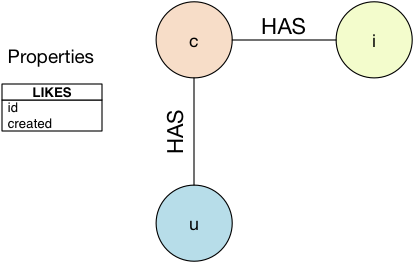
\includegraphics[width=2.5in]{img/edge_properties_has.png}
    \caption{ The {\tt has} relationship type example and attributes.}
    \label{fig:has}
\end{figure}

Is important to notice that this model is still partial view of the IEC system,
and other models can could be used in practice when implementing the system. 
For instance a relational database can be used for the implementation of a
user profile and authentication module. Also a copy or cache of the population 
could be kept in a key-value store in memory for performance reasons. 
Nevertheless, the model can give important insights of the behavior of the 
system.  

\section{Case Study}
\label{sec:experiments}

We present in this section the results of a comparison between two versions
of the same IEC application. The goal of the experiment is to compare two 
gamification techniques to increase volunteer participation. 
The main difference between both versions is how the fitness of individuals
is calculated and the information presented to users. 
\subsection{Gamification technique}
\label{sec:gamification}
The gamification technique
consists in giving more importance to the preference of users with more
participations. A feature found in video games is the concept of a 
score and experience levels. Levels depend on the score and certain features
of the game are only available to gamers when they reach a giving level.  

The score achieved by users depends on the actions he does in the system as
each time a user does one of these actions their score is incremented by one.
The actions considered in this application are: 
\begin{itemize}
\item Start a session.
\item Rate an individual.
\item Create a collection.
\item Save an individual of the wall to a collection.
\item Save an individual from a friend's collection.
\item Explore collections of other friends.
\end{itemize}
Only the "Start a session" and "Explore collections of other friends". 
Are not found in the graph model, 
%% Note: I must ask Christian where they're stored 
%%
Two scores are used to determine the weight of a user's preference:
\begin{itemize}
\item Experience. This value depends on the score and is a value 
between 0 and 100.

\item Participation. This value is simply the degree of the user node 
in the graph. This measure also considers the number of users he knows,
perhaps some of the users where invited to the system by him.   
\end{itemize}

Three versions were compared:
\begin{itemize}
\item Base (B). All users have the same weight.
\item Non Graph Gamification (G). Only experience is considered
\item Graph Gamification (GG) . Both experience and participation are considered.
\end{itemize}
When gamification was employed, all score values known where presented to users
and a ranking of users by weight was shown in a window, a screen capture of
this interface is shown in figure \ref{fig:top-users}. 

\begin{figure}[!t]
    \centering
        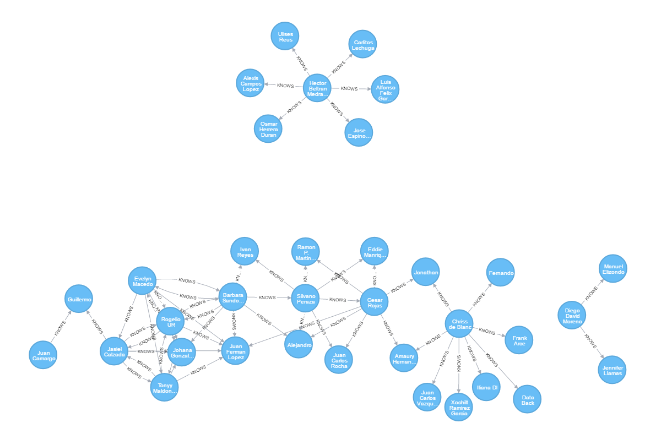
\includegraphics[width=3.5in]{img/user_known_2.png}
    \caption{Sample of users, showing the {\tt knows} relationship.}
    \label{fig:users-graph}
\end{figure}



\begin{figure}[!t]
    \centering
        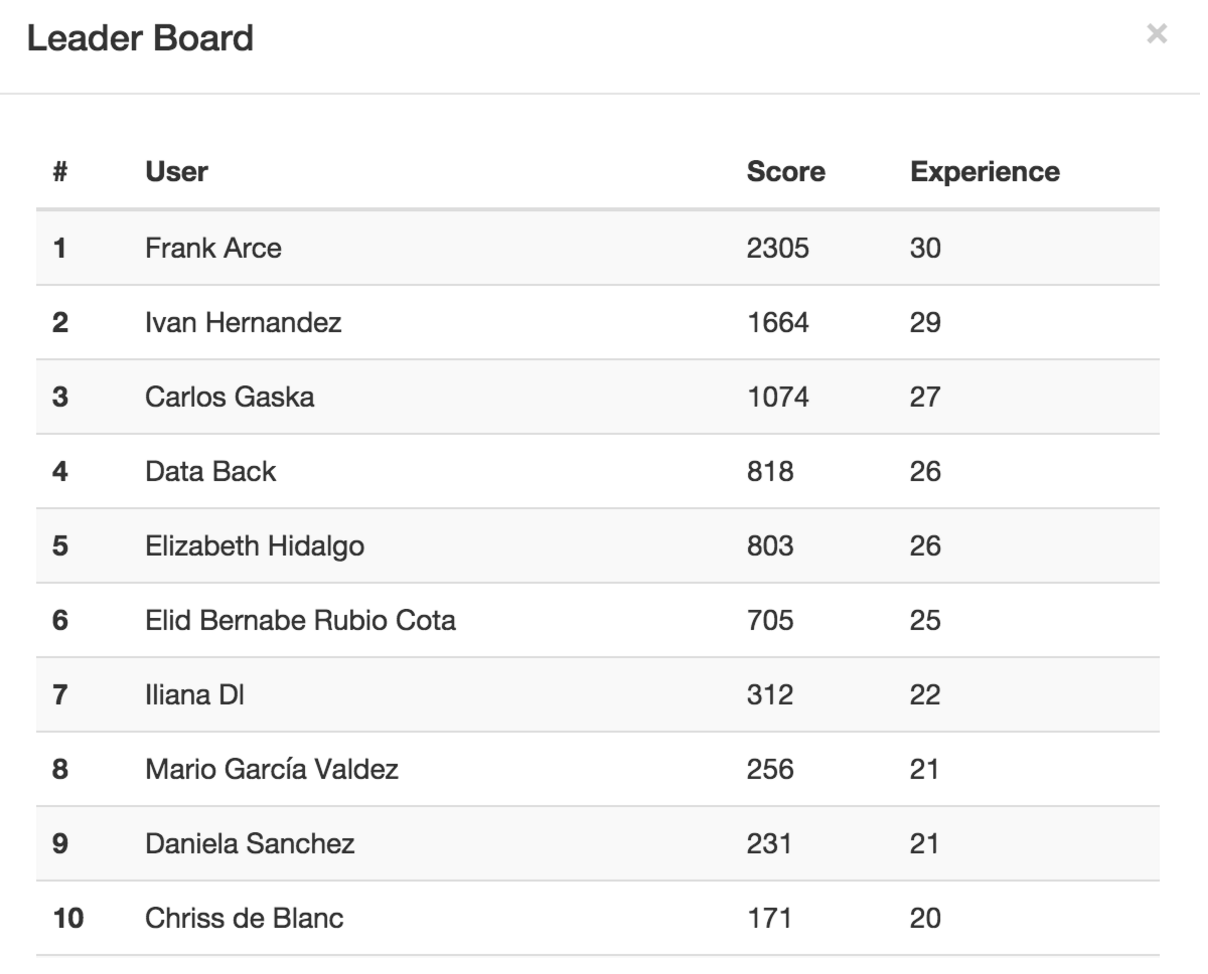
\includegraphics[width=3.5in]{img/leaderBoard.png}
    \caption{User interface showing top users.}
    \label{fig:top-users}
\end{figure}



\subsection{Set-up}
\label{sec:setup}

The three versions of the EvoDrawing web application were deployed to the
Heroku cloud service, using the same deployment configuration, using the
Heroku Free option with a 512 MB of RAM, adding only the GrapheneDB plug-in for the GG experiment.
Table \ref{tab:params} shows the parameters used for the evolutionary algorithm.

\begin{table}
  \small
  \caption{ Parameters for experiments.  }
  \label{tab:params} 
  \centering
  \small
  \begin{tabular}{l  c   }
    \hline\noalign{\smallskip}
     Parameter & Value \\
    \noalign{\smallskip}\hline\noalign{\smallskip}
    Initial Population Size   & 80 \\ \hline
    Sample Size & 1 \\ \hline
    Step Size & 8 Samples \\ \hline
    Mutation &  \\ \hline
    Selection & Tournament \\ \hline
    Tournament Size &  6 \\ \hline
  \end{tabular}
\end{table}
% Anuncements

http://goo.gl/jLis4Q


% Time
\subsection{Results}
\label{sec:results}

\begin{figure*}[!t]
    \centering
        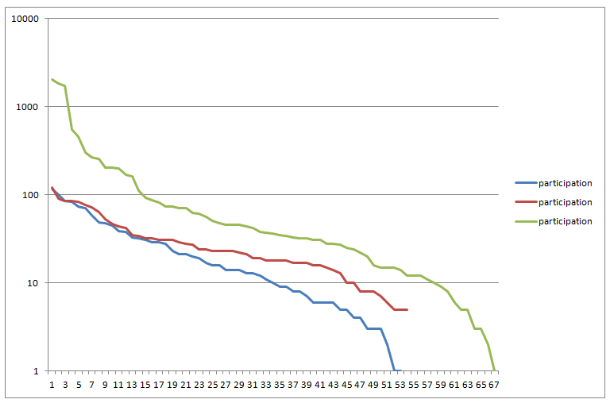
\includegraphics[width=3.5in]{img/comparison.png}
    \caption{Top ranked number individuals rated by user using a
     logarithmic scale.}
    \label{fig:top-ranked-participation}
\end{figure*}


\section{Conclusion}
\label{sec:conclusions}


\section*{Acknowledgment}


The authors would like to thank...





% trigger a \newpage just before the given reference
% number - used to balance the columns on the last page
% adjust value as needed - may need to be readjusted if
% the document is modified later
%\IEEEtriggeratref{8}
% The "triggered" command can be changed if desired:
%\IEEEtriggercmd{\enlargethispage{-5in}}

% references section

% can use a bibliography generated by BibTeX as a .bbl file
% BibTeX documentation can be easily obtained at:
% http://mirror.ctan.org/biblio/bibtex/contrib/doc/
% The IEEEtran BibTeX style support page is at:
% http://www.michaelshell.org/tex/ieeetran/bibtex/
%\bibliographystyle{IEEEtran}
% argument is your BibTeX string definitions and bibliography database(s)
%\bibliography{IEEEabrv,../bib/paper}
%
% <OR> manually copy in the resultant .bbl file
% set second argument of \begin to the number of references
% (used to reserve space for the reference number labels box)
\bibliographystyle{IEEEtran}
\bibliography{evospace-i,volunteer,biblio}

\end{document}


\end{document}


